\chapter{Introduction}

In this thesis, we explore certain aspects of the so-called high-temperature superconductors. While these materials were discovered fairly recently (1986), they have a rich history with hundreds of thousands of citations and, to this day, a lively debate surrounding the microscopic nature of this mysterious macroscopic quantum state. The purpose of this chapter is to briefly state the `the story so far' in broad strokes, and then dive deeper into state-of-the-art research relevant for the work performed in this thesis.

\section{Superconductivity}
Superconductivity is a state of matter where a material is able to conduct electricity with \emph{zero} resistance below a certain critical temperature $T_\text{c}$. Since we, fortunately, live in a world where the `spherical cow in a vacuum' model does not apply, it is remarkable to find \emph{real} materials where electrons can propagate without friction. In fact, experiments have shown, that under the right conditions it is possible to keep a persistent superconducting current running for 100000 years \cite{File1963}!

Superconductivity was first discovered in 1911 by Kamerlingh Onnes, essentially as a consequence of being able to liquefy helium in 1908 and reach temperatures close to absolute zero (see \cite{VanDelft2010} and references therein for a breakdown of the experiments). His low-temperature measurement of lead revealed a sudden drop in resistivity at \SI{4.2}{\kelvin}, as seen in the historic plot on figure \ref{fig:onnes}

\begin{figure}
    \centering
    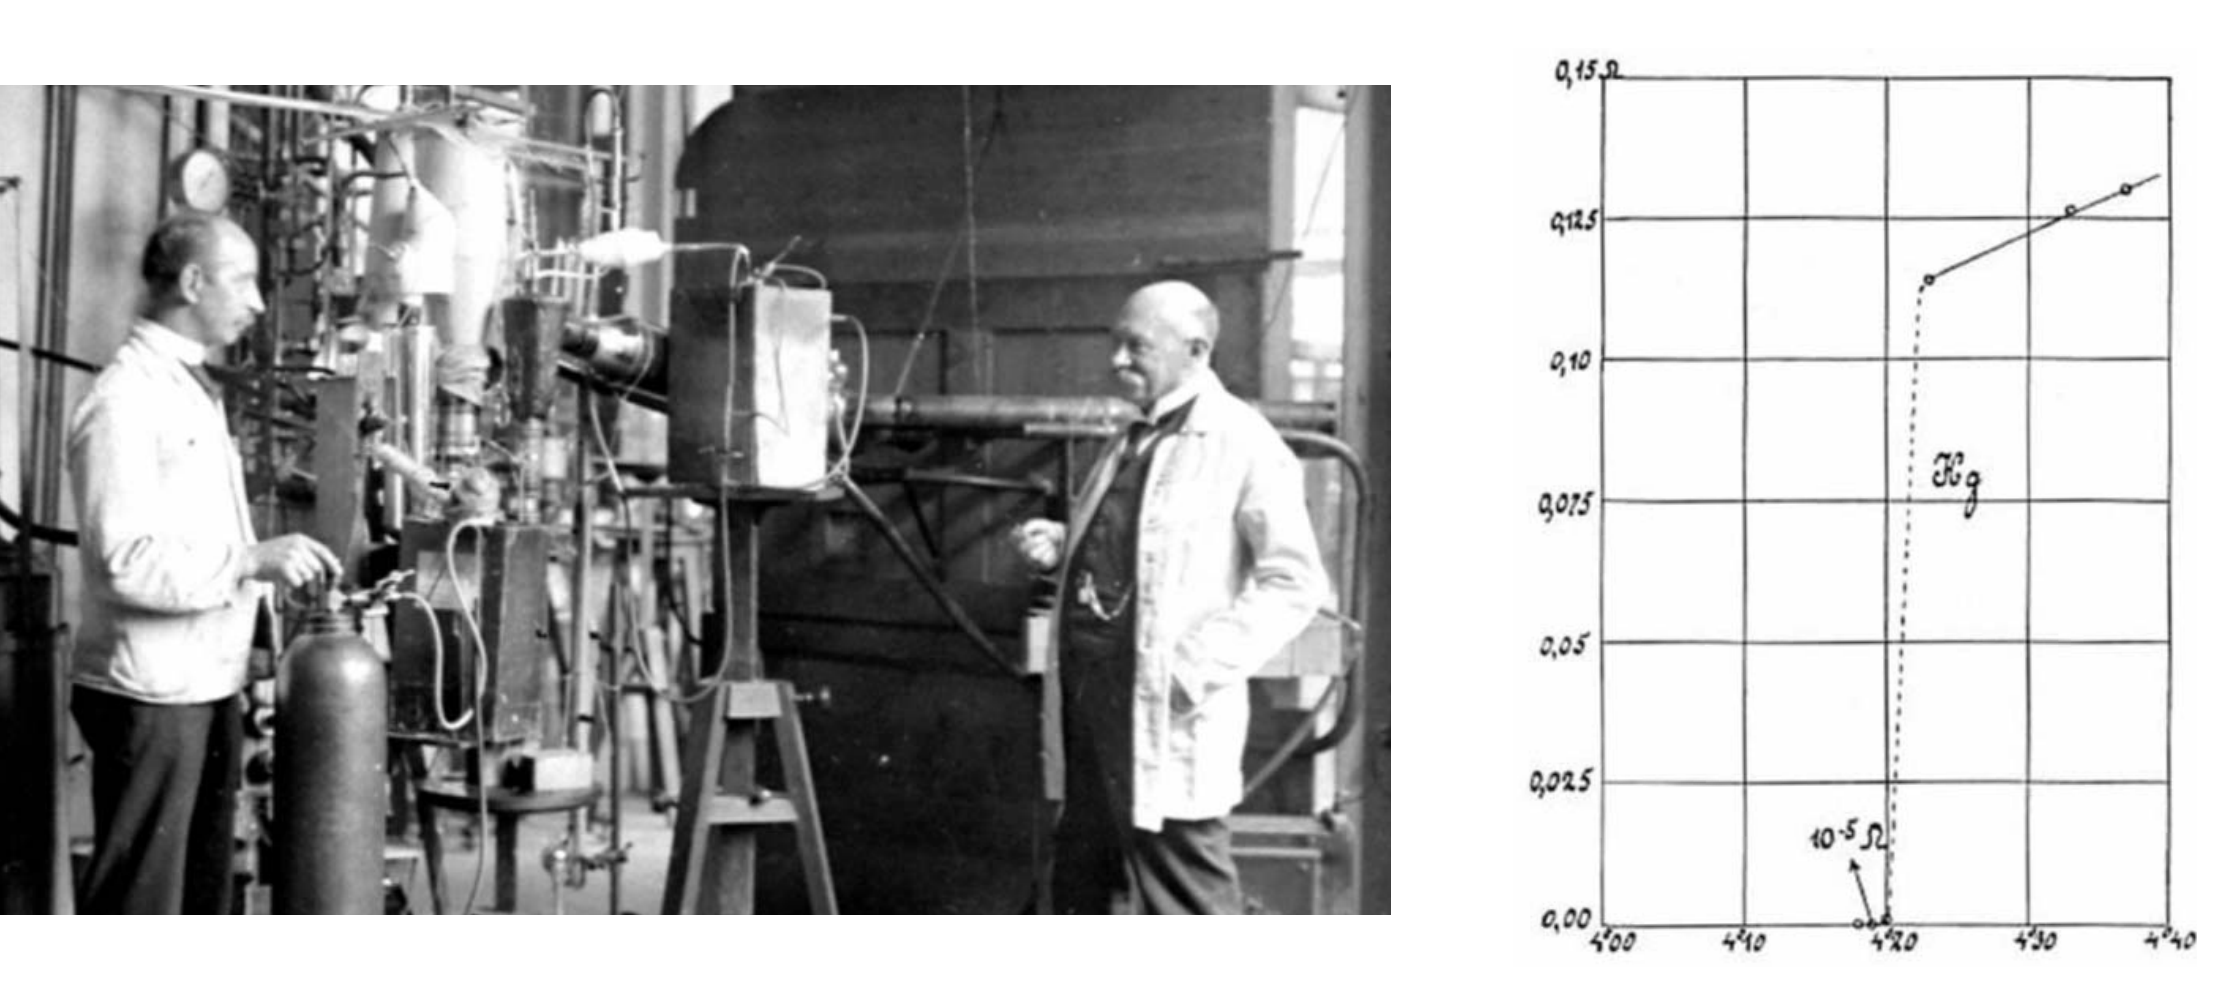
\includegraphics[width=\textwidth]{fig/intro/onnes.png}
    \caption{\textbf{Left}: Kammerling Onnes (right) and his chief engineer (left) in their cryogenics lab. \textbf{Right}: Resistivity as a function of temperature in elemental Lead. Both images from \cite{VanDelft2010}.}
    \label{fig:onnes}
\end{figure}

\begin{figure}
    \centering
    \missingfigure{Meissner effect}
    \caption{Meissner effect}
    \label{fig:meissner}
\end{figure}

Despite this remarkable experimental result, it would be 20 years for the next major milestone to appear. In 1933 the Meissner effect was discovered \cite{Meissner1933}, showing that superconducting materials would completely resist applied magnetic field by exhibiting perfect diamagnetism as sketched in figure \ref{fig:meissner}. In 1935 this effect was phenomenologically explained by the London equations, showing that the Meissner effect is due to superconducting currents on the surface of the material \cite{London1935}. From their relatively simple set of equations, an observable length scale known as the penetration depth was defined
%
\[ \lambda_\text{L} = \sqrt{\frac{m}{\mu_0 n q^2}} \, \]
%
where $\mu_0$ is the permeability of free space, $n$ the number concentration of the superconducting carriers, $m$ the electron mass and $q$ the electron charge. This length scale determines how an external magnetic field penetrates the superconductor through the relationship $B(x) = B(0) \exp (-x / \lambda)$. $\lambda$ is typically on the order of \SIrange{20}{100}{\nano\meter} \cite{Kittel2005}.

Another roughly 20 years would pass until Landau's work on phase transitions paved the way to understanding the superconducting phase transition as a thermodynamic quantity through the Ginzburg-Landau equations in 1950 \cite{Ginzburg2009}. I will not repeat the details here, but the idea is to make a polynomial expansion of the free energy as a function of a complex superconducting wavefunction $\psi$. As the material is cooled below $T_\text{c}$, $\psi$ `choses' a phase and breaks gauge symmetry, analogous to how a ferromagnet choses a common direction for the magnetic moment at the magnetic phase transition. This description predicts an new characteristic length scale of the superconductor called the \emph{coherence length} $\xi$ and recasts the penetration depth in terms of $\psi$:
%
\[ \xi = \sqrt{\frac{\hbar^2}{4m|\alpha|}} \qquad \lambda = \sqrt{\frac{m}{4\mu_0 e^2 \psi_0^2 }} \, , \]
%
where $\alpha$ is a phenomenological parameter of the polynomial expansion. The ratio of these parameters, $\kappa = \lambda / \xi$, are used to classify superconductors into type-I ($\kappa < 1 / \sqrt{2}$) and type-II ($\kappa > 1 / \sqrt{2}$). The significance of $\kappa > 1 / \sqrt{2}$ can be understood as a threshold where the surface tension between normal and superconducting phases becomes negative \cite{Abrikosov1957}. Intuitively, the coherence length $\xi$ defines the shortest length within which the superconducting carrier concentration are allowed to change considerably. For elemental metals $\xi$ can be up to a micrometre: \SI{1600}{\nano\meter} in Al and \SI{83}{\nano\meter} in Pb \cite{Kittel2005}. In the cuprates (which will be discussed in detail in the next section), $\xi$ is typically on the order of a few lattice spacings (\SI{1}{\nano\meter} in YBa$_2$Cu$_3$O$_{7-\delta}$ \cite{Tomimoto1999}).

Based on Ginzburg-Landau theory, \citeauthor{Abrikosov1957} predicted the existence of vortices in Type-II superconductors, which showed excellent agreement with the measured magnetization of several lead alloys \cite{Abrikosov1957}. These vortices can be pinned by defects and form a lattice that we have been able to image using modern day microscopy techniques (see e.g. \cite{Wells2015} for a recent example with beautiful real-space images). The experimental evidence piled up \cite{Doll1961, Deaver1961}, and it quickly became evident that Ginzburg-Landau theory is applicable to most known superconductors, including the cuprates and iron-based varieties.

Despite the descriptive power of Ginzburg-Landau theory, we are left with no recipe on how to construct, even theoretically, `better' superconductors. In order to manipulate material properties, it is necessary to understand the microscopic properties that lead to macroscopic behaviour (e.g. how phonons influence thermal properties or how magnetic exchange influence magnetic properties. Inspired by Ginzburg-Landau theory, rapid progress towards a microscopic theory was being made in the mid 1950s, culminating in the famous BCS theory formulated by Bardeen, Cooper and Schrieffer \cite{Bardeen1957}. 

BCS theory is based on the assumption that an attractive interaction between electrons at the Fermi level can result in so-called `cooper-pairs', a bosonic quasi-particle consisting of an electron pair of opposite momentum and spin. The bosonic nature of this quasi-particle can, at low temperatures, result in a Bose-Einstein condensate where a large fraction of these electron pairs occupy the lowest energy quantum state. This microscopic theory of superconductivity made several testable predictions, such as the appearance of an energy gap with a temperature-dependent width $\Delta(T)$ in the electronic density of states related to the critical temperature through the relationship
%
\[ 2\Delta(T=0) = 3.5 k_\text{B} T_\text{c} \, , \]
%
where $k_\text{B}$ is the Boltzmann constant. A few years later electron tunnelling experiments confirmed this prediction with reasonable accuracy \cite{Giaever1960, Giaever1960a}. Additionally, \citeauthor{Josephson1962} predicted that superconducting currents could tunnel across an insulating a barrier \cite{Josephson1962}, experimentally verified a few years later \cite{Jaklevic1965}.

While BCS theory predicts an attractive interaction between electrons, the original paper \cite{Bardeen1957} makes no assumption about the nature of this interaction. Some experiments, performed a few years prior, showed that $T_\text{c}$ of Hg$^{198}$ was higher when compared to that of natural Hg (avg. atomic weight of 200.6) \cite{Maxwell1950, Reynolds1950}. Since the chemistry of these materials can be assumed identical, this experiment suggests a positive correlation between phonon frequencies and $T_\text{c}$, since lighter elements have more energetic vibrations. Assuming an attractive potential due to lattice vibrations, BCS theory could relate the attractive interaction to phonon frequencies and predict a relative relationship between isotopic mass and critical temperature \cite{DeLaunay1954}:
%
\[ T_\text{c} \propto \frac{1}{\sqrt{m_\text{ion}}} \, , \]
%
where $m_\text{ion}$ is the isotopic mass of the constituent ionic species. With BCS theory, superconductivity in many elemental metals were believed to be `solved' with the identification of phonon-mediated superconductivity. Unfortunately, this discovery also set a \emph{practical} upper limit on $T_\text{c}$. In order to increase phonon frequencies, and thus critical temperatures, we need materials with low mass atomic species, while still being crystalline. At ambient pressure this practical upper limit is often quoted to be around \SI{30}{\kelvin}. A good demonstration of this principle is actually a counter-example where researchers were able to reach a critical temperature of $T_\text{c} = \SI{200}{\kelvin}$ by applying a pressure of \SI{155}{\giga\pascal} to H$_2$S \cite{Drozdov2015}. This material contains the light atomic species we require, but cannot crystallize at ambient pressures so we can only reach high critical temperatures under extreme conditions. A different example is the highly unusual case of MgB$_2$, where coincidences add up to an unusually high electron-phonon coupling resulting in a critical temperature of $T_\text{c} = \SI{39}{\kelvin}$ \cite{Nagamatsu2001}.

While this thesis has nothing to do with BCS superconductors and, in principle, could have been written without ever mentioning them, I believe that the history of conventional superconductivity emphasises exactly what is desired from a `solution' to high-temperature superconductivity. It is also a fascinating story due to the fact that the tools to solve the problem were not even close to being developed when the phenomenon was discovered. It took roughly 50 years for a satisfying conclusion and we have only been working on the cuprates for roughly 30 years. 

\section{Cuprates}
With this brief introduction to superconductivity, I will proceed with an introduction to cuprate superconductivity. While the previous section was at least moderately complete, it is impossible to capture an unbiased view of cuprate research. As such, the following will be somewhat narrowly focussed. While this is a reasonable choice for this introduction, it is important to realize just how massive the field is and how impossible it is to know every last detail. That being said, I have thoroughly enjoyed exploring the vast literature and I will recommend anyone reading this to do the same.

Before we begin, I want to get some of the nomenclature out of the way. As the title of this thesis suggest, I am working on the so-called `high-temperature superconductors'. This definition essentially only concerns itself with the value of the critical temperature (usually above the `BCS-limit' of \SI{30}{\kelvin}), without saying anything about other physical properties. On the other hand Type-I and Type-II, as seen in the previous section, are rigidly defined with respect to their properties as defined through Ginzburg-Landau Theory. Finally, `conventional superconductors' are those that can be microscopically described with BCS theory, while 'unconventional superconductors' cannot. While cuprates are relatively simple crystals, most of them have a variety of names and abbreviations attached to them. Table \ref{tab:cuprates} lists the most important ones along with their critical temperatures and a few other physical properties.

\begin{table}
    \caption{list of cuprates}
    \label{tab:cuprates}
    \missingfigure{Table of cuprates, formulae, names, Tc, crystal structure}
\end{table}

\subsection{The discovery of LBCO}
Roughly 30 years after BSC theory, in 1986, Bednorz and M\"uller discovered a new type of superconductor while trying to manipulate the electronic properties of the anti-ferromagnetic insulator La$_2$CuO$_4$. By effectively removing a small number of electrons from the system by substitution of dopant species, they achieved a record $T_\text{c}$ of \SI{30}{\kelvin}. Shortly after, in 1987, the sister-compound YBa$_2$Cu$_3$O$_{7-\delta}$ was discovered, shattering previous records and finally achieving a critical temperature $T_\text{c} = \SI{93}{\kelvin}$ that could be reached using liquid nitrogen \cite{Wu1987}.

While the increased critical temperatures are remarkable on their own, it quickly became apparent that we were dealing with a completely new type of superconductivity which cannot be explained with BCS theory. The normal state ($T > T_\text{c}$) of cuprate superconductors is as, if not more, complex when compared to the superconducting state and the BCS assumption of being metallic in the normal state is generally not fulfilled. In addition, the BCS relationship between isotopic mass critical temperature ($T_\text{c} \propto m_\text{ion}^{-0.5}$) is not fulfilled when performing O$^{16}$/O$^{18}$ isotopic substitution \cite{Suryadijaya2005}.

Similar to semiconductors, the properties of the cuprates are dramatically changed with the introduction of dopant species. In general, we call the addition of electrons \emph{electron doping} and the removal of electrons \emph{hole doping}. In the original paper, La$_2$CuO$_4$ was hole-doped by exchanging La$^{3+}$ with Ba$^{2+}$. We define the amount of hole-doping ($n_\text{h}$) is the fraction of substituted atomic species per formula unit. The amount of electron doping ($n_\text{e}$) is defined similarly. In general, the undoped compounds $n_\text{h} = 0$ are antiferromagnetic insulators and you need a small amount of doping to make the materials superconducting. Too much (typically $n_\text{h} > 0.25$) and the materials become non-superconducting metals. 

The fact that we need finite amounts of doping in order to make cuprates superconducting, makes them inherently inhomogeneous materials. This inhomogeneity may or may not be important for cuprate superconductivity, but there is no denying that it exists. In fact, recent STM studies on Bi$_2$Sr$_2$CaCu$_2$O$_8+\delta$ have shown significant spatial inhomogeneities due to random distributions of defects \cite{Ruan2018}. If this inhomogeneity is relevant, it presents us with a great difficulty in producing models that can explain superconductivity; adding too much complexity can be detrimental to explanatory power (Occam's razor).

\subsection{Structure}
Cuprate superconductors are characterized by a layered structure where CuO$_2$ layers are separated by so-called charge reservoirs (or spacer layers). In general, the conventional Bravais lattice is either tetragonal or orthorhombic with the CuO$_2$ layers in the $a$-$b$ plane. A few examples of cuprate crystal structures is shown in figure \ref{fig:cuprate_family_structures}. The different structures are generally characterized by the number $n$ of subsequent CuO$_2$ layers. Interestingly, increasing $n$ generally improves the critical temperature $T_\text{c}$ up to $n = 3$. It has been suggested that the decrease at $n \geq 3$ could be due to the fact that the `inner' and `outer' CuO$_2$ layers cannot reach similar doping.

\begin{figure}
    \centering
    \missingfigure{selection of cuprate crystal structures, LSCO on the left}
    \caption[various cuprate structures]{various cuprate structures}
    \label{fig:cuprate_family_structures}
\end{figure}

Doping is performed either by substitution or addition of dopant species as indicated by figure \ref{fig:cuprate_family_structures}. Doping thus necessarily changes the lattice either due to a difference in ionic radii of a substitutional dopant or a strain in the lattice because of an interstitial species. Since the interstitials are almost\todo{I thinkt it might be allways?} always oxygen atoms, these effects are mostly seen when varying substitutional dopant of different atomic radii. In the case of substitutional doping of La$_2$CuO$_4$, the structural and electronic properties vary wildly (as we shall see in section \ref{sec:lsco}) depending on the dopant species (Ba, Sr).

Different members of the cuprate family have their own structural peculiarities. In single-layer LSCO, many structural properties are linked to the CuO$_6$ octahedra not present in structures with $n \geq 2$ and In YBCO, Cu-O chains form along the crystallographic $b$-axis. Despite these specific structural properties of the various cuprates, they are all equipped with square-planer CuO$_2$ planes and have remarkably similar (electronic) phase diagrams.

\subsection{Phase diagram}
A general phase diagram for the cuprates is shown in figure \ref{fig:cuprate_phase_keimer} illustrating the many macroscopic and microscopic phases in the cuprates as a function of temperature and doping. First, figure \ref{fig:cuprate_phase_keimer} (left) shows an unexpected asymmetry between hole and electron-doping. Since cuprates are superconducting for a wider range of doping on the hole-doped side, most research focusses solely on this side of the phase diagram\todo{Other arguments? More discussion of the assymetry?}. Second, as shown in figure \ref{fig:cuprate_phase_keimer} (right), cuprates are only superconducting for a narrow range of hole doping typically between $n_h = 0.05$ and $n_h = 0.25$ with a maximum around $n_h = 0.15$. This region is known as the `superconducting dome'. 

\begin{figure}
    \centering
    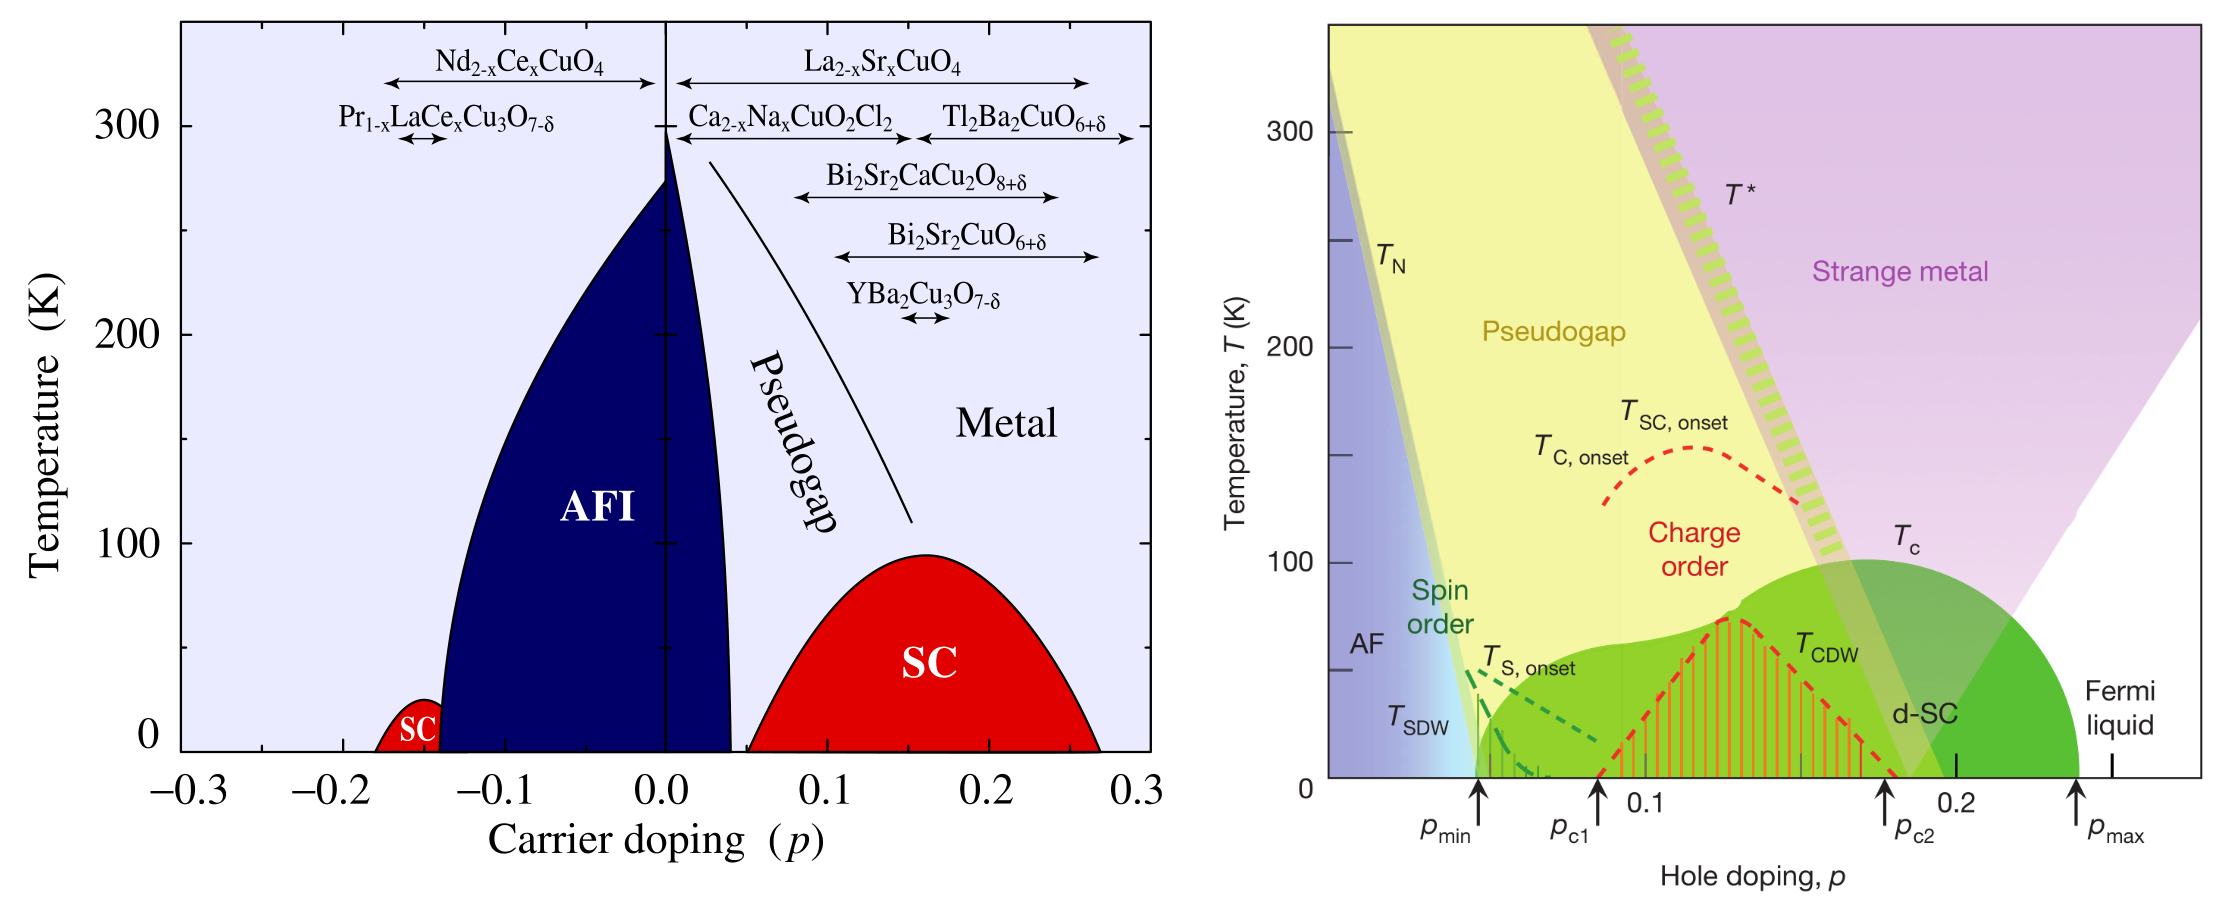
\includegraphics[width=\textwidth]{fig/intro/keimer.png}
    \caption[cuprate phase diagrams]{\textbf{Left:} Generalized phase cuprate phase diagram for selected electron- and hole-doped materials, emphasizing the asymmetry between the two sides of the phase diagram. From \cite{Peets2007}. \textbf{Right:} Generalized phase diagram for the hole-doped side annotated with microscopic ordering phenomena. From \cite{Keimer2015}.}
    \label{fig:cuprate_phase_keimer}
\end{figure}

I emphasize here the very different states of matter at the boundaries of the superconducting dome at $T=0$; over-doped cuprates are typically metals while underdoped cuprates are magnetic insulators. In some sense, superconductivity is optimized in a region between localized (magnet) and itinerant (metal) behaviour -- a region also containing poorly understood normal state ($T > T_\text{c}$) behaviour such as the Pseudogap and strange metal phase.

The Pseudogap is a curious phenomena first observed in NMR measurements of YBCO \cite{Alloul1989} and later on in the $c$-axis resistivity \cite{Homes1993} and specific heat \cite{Loram1993}. The name comes from the fact that, by now, it is generally associated with the opening of a gap in the electronic density of states (see below). The difficulty in finding a microscopic origin of the phase transition at the Pseudogap temperature $T^*$ has attracted as much attention as the superconducting transition itself. Many researchers believe that the key to understanding the superconducting transition is directly related to the Pseudogap. One idea is that of `pre-formed pairs', where Cooper pairs start forming at $T^*$, but the macroscopic superconducting state fails to settle between $T^*$ and $T_\text{c}$ due to incoherent fluctuations in the phase of the pairing field ($\psi$ in Ginzburg-Landau theory) \cite{Emery1995, Curty2003}.\todo{maybe remove this last bit, too technical}

The strange metal phase is possibly the least understood part of the cuprate phase diagram \cite{Keimer2015}. A `strange' metal is essentially a phase of matter where the theory of `normal' metals (fermi liquids) breaks down and is a phenomenon seen in a number of correlated electron systems, not just the cuprates. A significant indicator of this behaviour is a linear temperature-dependence of resistivity (see e.g. \cite{Martin1990} for a cuprate example), where a normal fermi liquid varies as $T^2$ at low temperatures. A recent study even suggests that linear-in-$T$ resistivity in the cuprates is a generic property related to a universal scattering rate \cite{Legros2018}.

By outlining the the phase diagram in this way, I intend to illustrate both the difficulty of solving the cuprate problem and the many experimental methods and theoretical tools necessary to investigate the various features of this complex phase diagram. Until now, apart from crystallographic information, we have mainly considered \emph{macroscopic} behaviour through bulk measurements such as resistivity, specific heat, optical band gap or magnetic susceptibility. We now turn to a brief overview of \emph{microscopic} behaviour, starting with momentum-resolved measurements of the fermi surface.

\subsection{Fermi Surface}
Angle-Resolved Photoemission Spectroscopy (ARPES) is a method in X-ray spectroscopy that directly probes the electronic band structure of materials. This method has been extremely important in strongly correlated electron systems in general and has a rich history with the cuprates (see the extensive review by \citeauthor{Damascelli2003} \cite{Damascelli2003}).

\subsection{Microscopic correlations}
The primary method for investigations in this thesis is inelastic neutron scattering (INS), which will be covered extensively in chapter \ref{ch:method}. For now, we just briefly state some of the things that can be measured by this and related methods.

\section{Lanthanum Based Cuprates}\label{sec:lsco}
In this section, we look more closely at the Lanthanum based cuprates. These are variants of the material discovered by Bednorz and M\"uller all based on the La$_2$CuO$_4$ parent compound (leftmost compound on figure \ref{fig:cuprate_family_structures}). Sometimes known as `La214' or with specific acronyms depending on the dopant species, these materials are single-layer cuprates with a relatively simple crystal structure and a maximum critical temperature $T_\text{c} \approx \SI{40}{\kelvin}$.

Since this thesis is focussed on specific structural aspects and phonon dynamics, this `relatively' simple crystal structure is a particularly strong point for us. Since we want to model the full 3-dimensional structure using computationally heavy simulation methods, it is advantageous to consider the simplest system possible. In addition, since the lanthanum cuprates were the first so-called 'high-temperature superconductors` to be discovered, there is a massive amount of literature on which to build our ideas from.  

In the phase diagram presented in figure \ref{fig:cuprate_phase_keimer}, a few of the many phenomena in the cuprates were indicated. In this section we will discuss these phenomena specifically in the context of lanthanum cuprates and relate them to other compounds where applicable. 


\begin{figure}
    \centering
    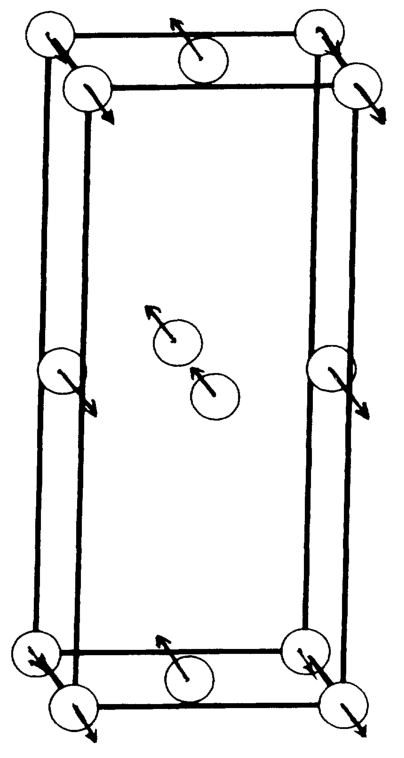
\includegraphics[width=0.3\textwidth]{fig/lsco/lsco_afm.png}
    \caption[AFM structure of LSCO]{AFM structure of LSCO}
    \label{fig:lsco_afm}
\end{figure}

\section{LSCO+O}

\section{Thesis objectives}
